\newpage
\section{Question 1}
\subsection{Problem:}
Assume that all processes in the system have similar behavior, where a process spends ½ of its time
performing I/O and ½ of the time performing execution. The system is capable of overlapping execution
time for a process with I/O time of another. The system is utilizing also RR for scheduling with a time
quantum of 3ms (ignore context switch time; i.e. assume it takes 0 ms). Show the Gantt Chart for all your
answers.

\subsection{Part A }
\subsubsection{Best CPU utilization}

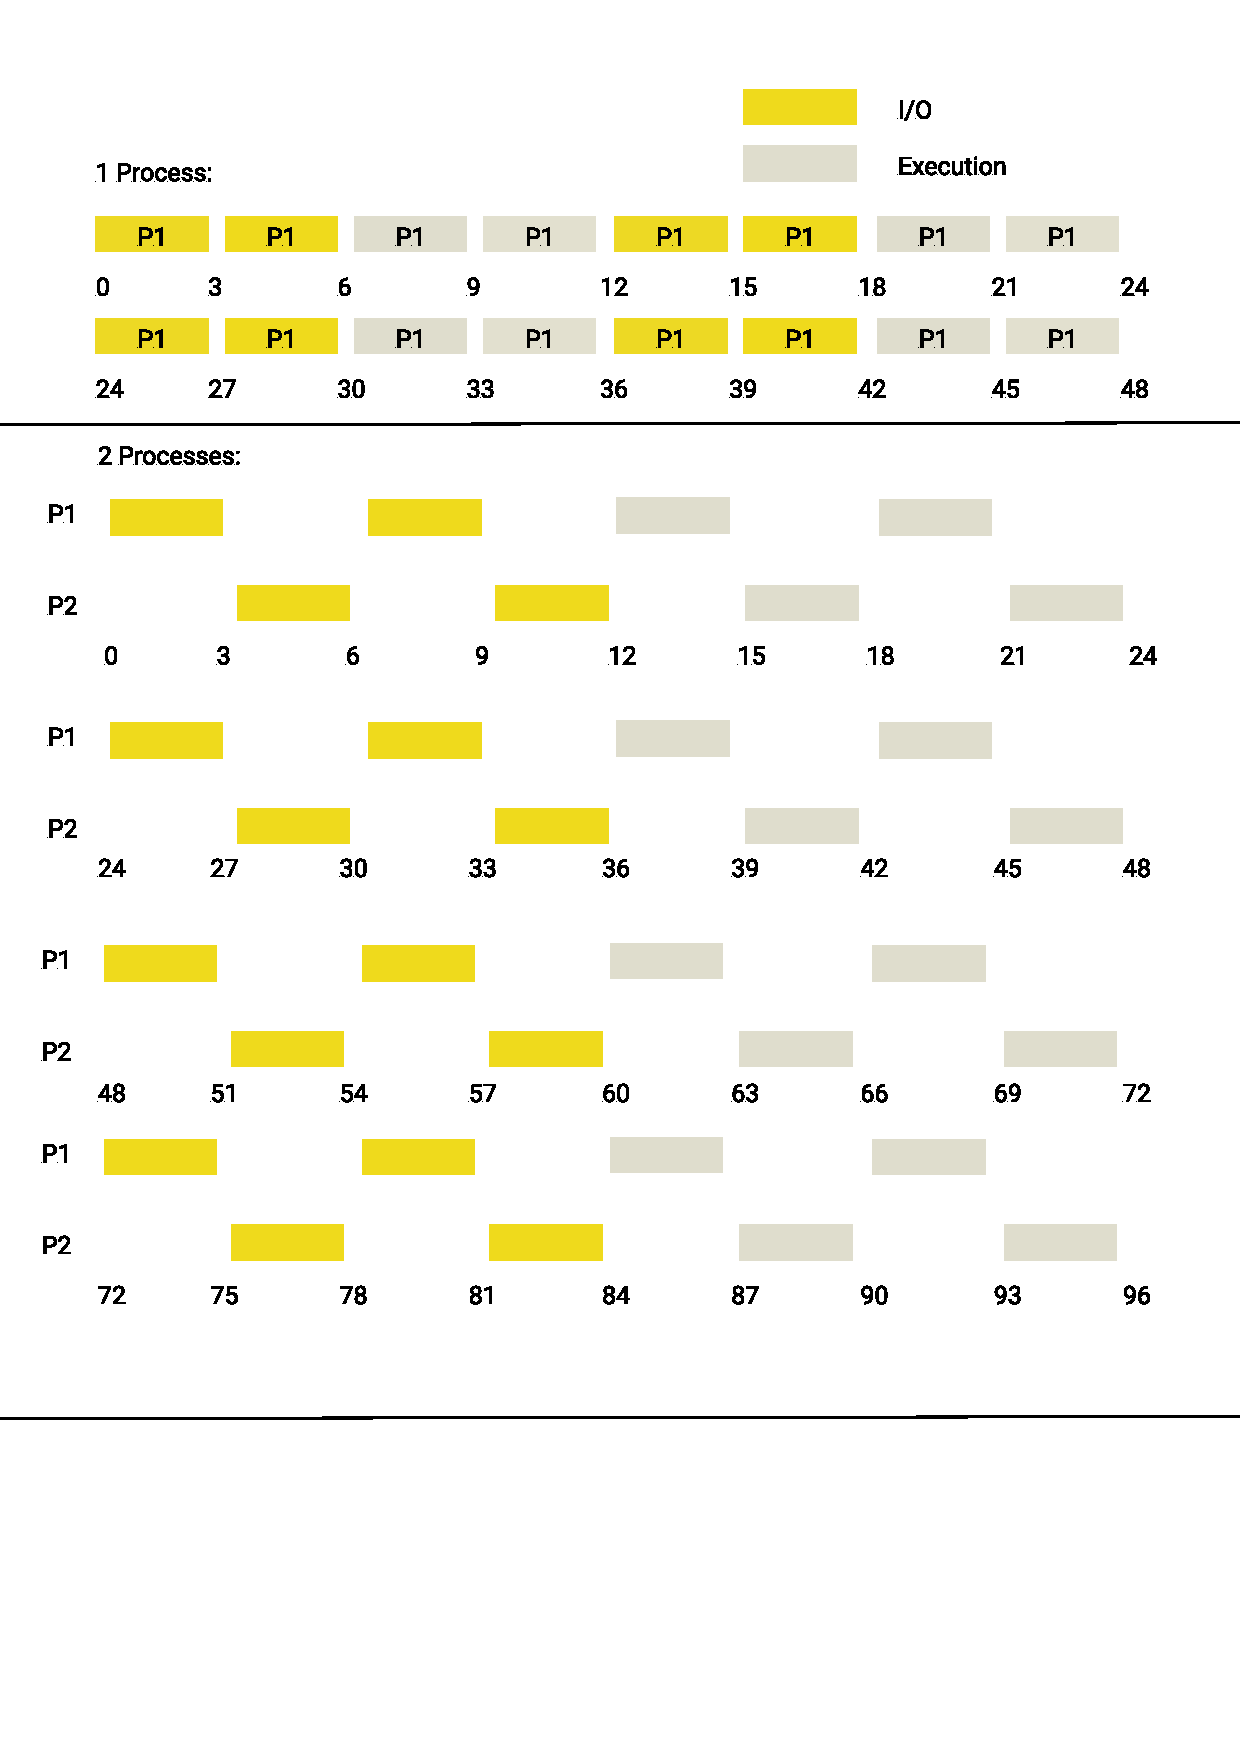
\includepdf{Q_1A}

\begin{itemize}
    \item With 1 process running, CPU utilization = $\frac{24}{48} * 100\% = 50\%$
    \item With 2 processes running, CPU utilization = $\frac{48}{96} * 100\% = 50\%$
\end{itemize}

\subsubsection{Throughput if 2 processes are running}
\begin{align*}
    \text{throughput} = \frac{2}{96} \approx 0.02083 \text{ (process) }
\end{align*}


\subsection{Part B }
